\documentclass[a4paper, 12pt]{article}

\usepackage[top=2cm, bottom=2cm, left=2.5cm, right=2.5cm]{geometry}
\usepackage[utf8]{inputenc}
\usepackage{array}
\usepackage{graphicx}
\usepackage{listings}
\usepackage{caption}
\usepackage{float}
\usepackage[labelfont=bf]{caption}

\captionsetup[lstlistings]{position=bottom}
\graphicspath{{img/}}

\begin{document}
\lstset{language=SQL}
\textbf{UNIVERSIDADE TECNOLÓGICA FEDERAL DO PARANÁ | UTFPR} \\
\textbf{ALUNO:} Ricardo Medeiros da Costa Junior   \textbf{RA:} a1598996 \\
\textbf{DISCIPLINA:} Banco de Dados para Biologia \\
\textbf{ATIVIDADE:} Sistema de Recomendações | Tarefa 3 

\section{Persistência dos dados}
O organismo selecionado para a importação foi o \emph{Anaerococcus Lactolyticus}. Foi realizado a importação com a seguinte consulta:

\begin{lstlisting}[frame=single]
using periodic commit 600
load csv with headers from
'file:/Users/cleversonbarbosanalesso/Downloads/
anaerococcus_lactolyticus.csv' as l fieldterminator ' '
merge (p1: Protein {protein: l.protein1})
merge (p2: Protein {protein: l.protein2})

merge (p1)-[r\:INTERACTS_WITH]-(p2)
      on create set r.combined_score = toFloat(l.combined_score),
        r.neighborhood = toFloat(l.neighborhood),
          r.fusion = toFloat(l.fusion),
            r.cooccurence = toFloat(l.cooccurence),
                  r.homology = toFloat(l.homology),
                  r.coexpression = toFloat(l.coexpression),
                    r.experimental = toFloat(l.experimental),
                      r.knowledge = toFloat(l.knowledge),
                  r.textmining = toFloat(l.textmining)
order by person.name
\end{lstlisting}

Utilizou-se o \emph{using periodic commit 600} para evitar problemas referentes a gerenciamento de memória, conforme sugere a documentação oficial do \emph{Neo4j}. O número 600 é a quantidade de registros por \textit{commit}. \\

Criou-se um índice, para melhorar a performance das consultas:

\begin{lstlisting}[frame=single]
CREATE INDEX ON :Protein(protein)
\end{lstlisting}

Após realizado a importação, foi consultado a quantidade de nós e relações e foi exibido as informações do sistema para verificar se a importação ocorreu sem erros. Conforme demonstrado na Figura 1 e 2.

\begin{figure}[H]
  \centering
  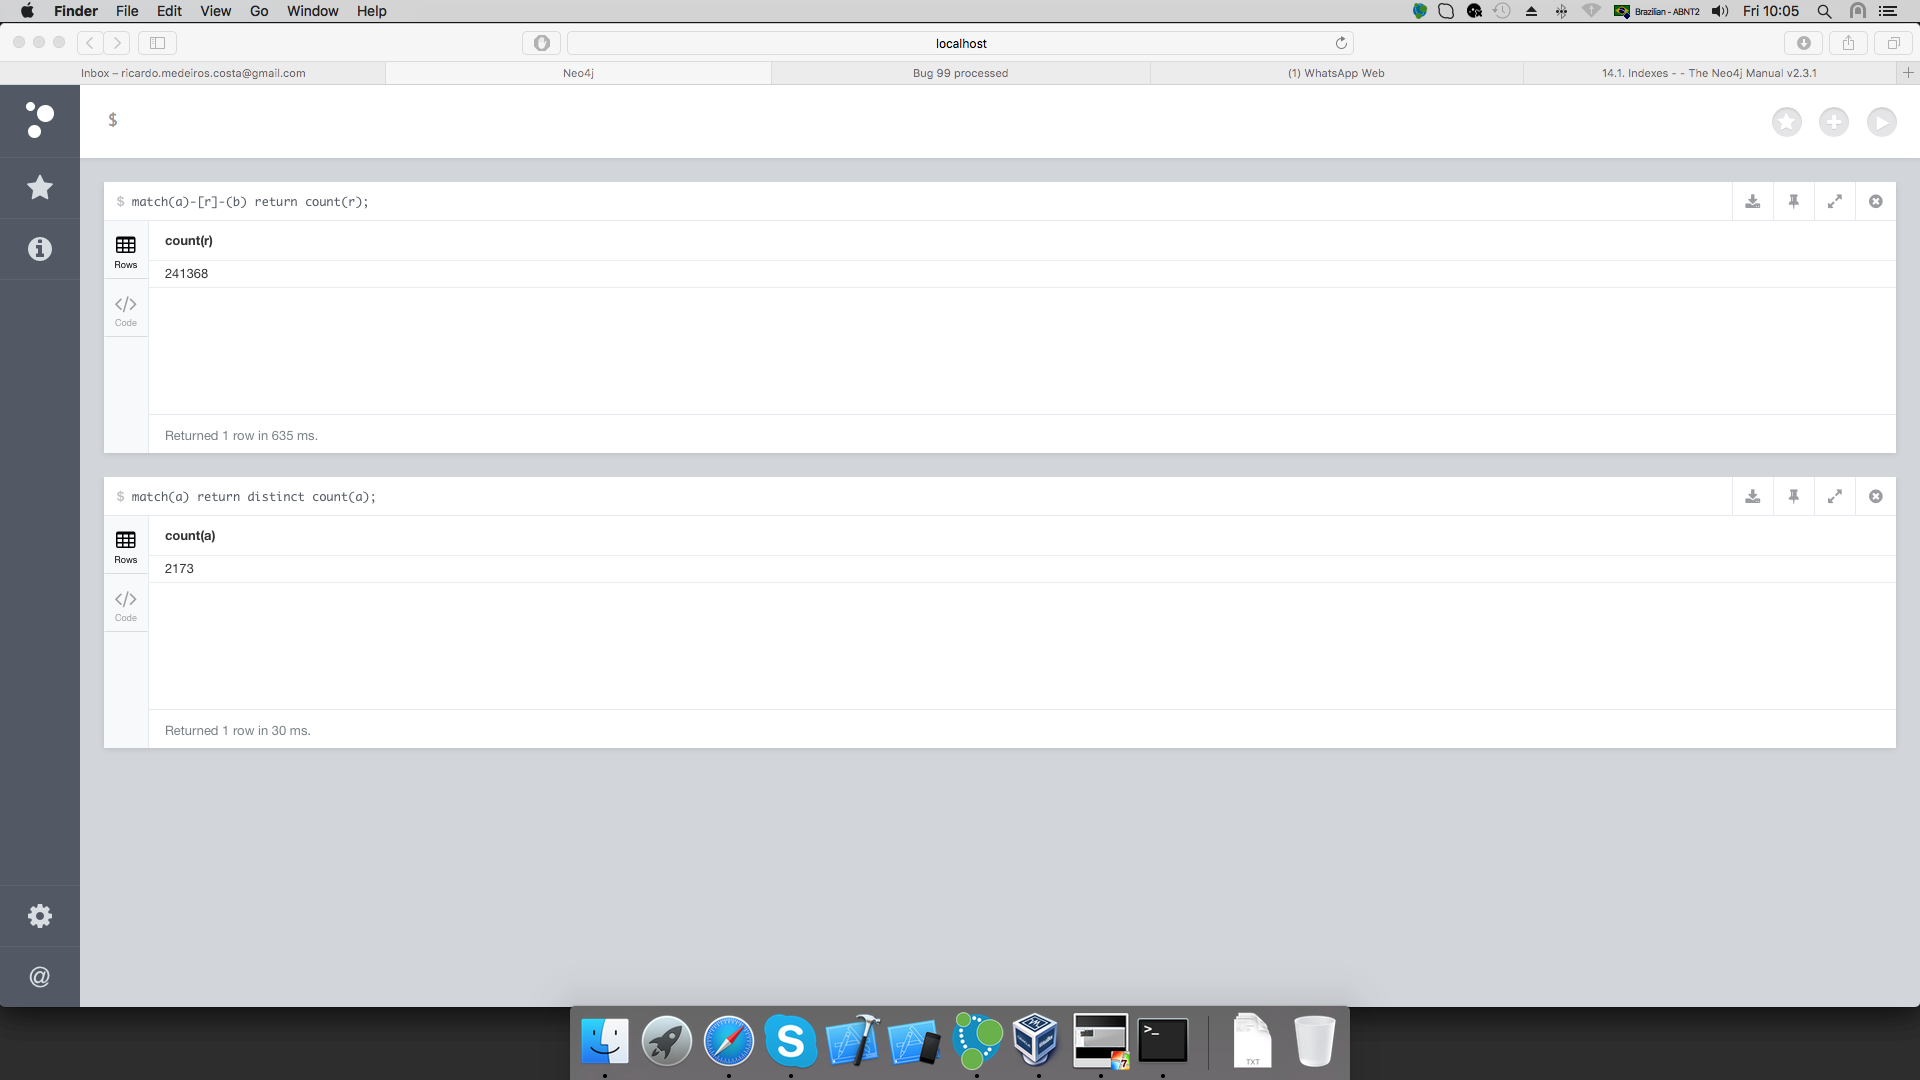
\includegraphics[width=1\textwidth]{1}
  \caption[1 - Quantidade de nós e relações]{\textbf{Quantidade de nós e relações}}
\end{figure} 

\begin{figure}[H]
  \centering
  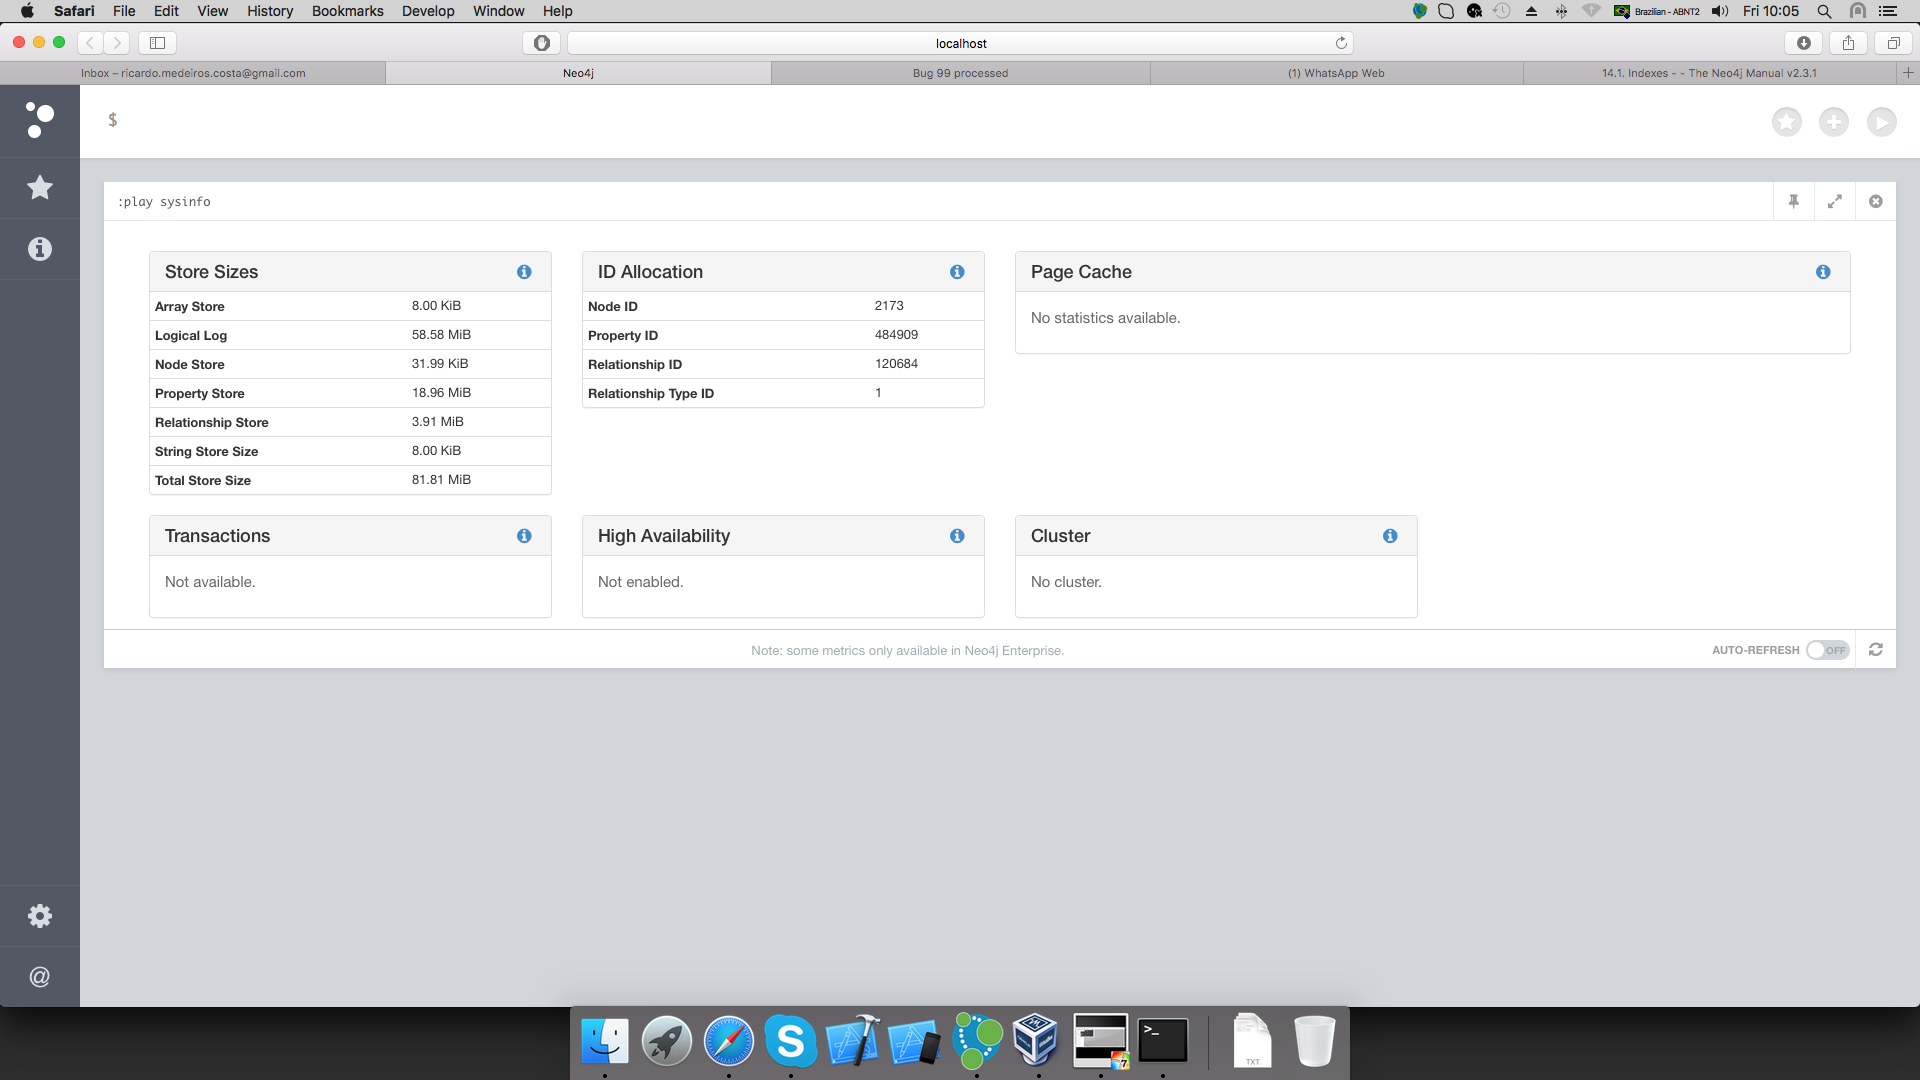
\includegraphics[width=1\textwidth]{2}
  \caption[2 - Informações do sistema]{\textbf{Informações do sistema}}
\end{figure}

O banco criado possui 2.173 nós e 241.368 relações.

\section{Listando Interações pelo Combined Score}

\begin{lstlisting}[frame=single]
match(a)-[r]-(b)
return a.protein, b.protein, r.combined_score
order by r.combined_score desc;
\end{lstlisting}

O resultado: 
\begin{figure}[H]
  \centering
  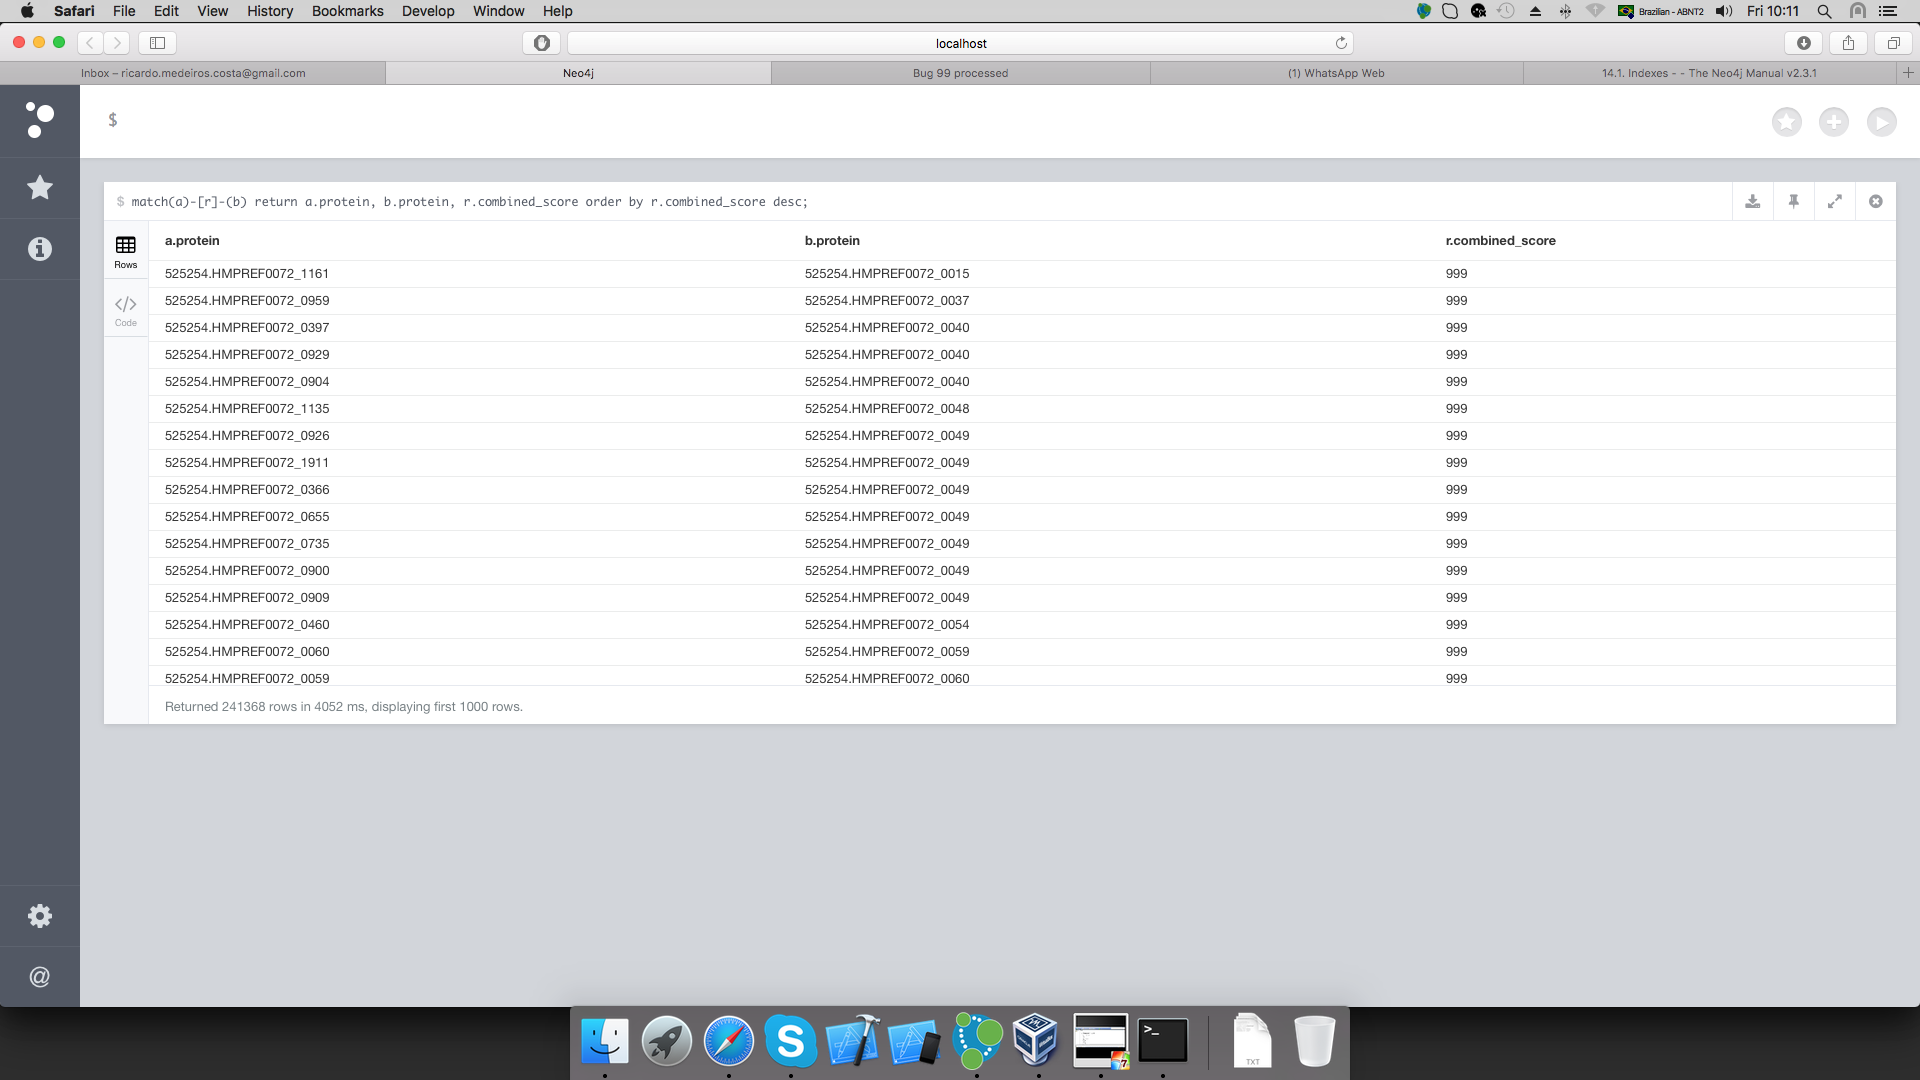
\includegraphics[width=1\textwidth]{3}
  \caption[3 - Listando Interações pelo Combined Score]{\textbf{Listando Interações pelo Combined Score}}
\end{figure} 

\section{Filtrando Interações}
Foi adicionado nessa consulta a cláusula \emph{limit 400}, com objetivo de ser exibido apenas 400 resultados para facilitar a visualização.

\begin{lstlisting}[frame=single]
match(p1)-[r]-(p2)
where r.textmining > 0.95
return p1, r, p2 limit 400;
\end{lstlisting} 

O resultado: 
\begin{figure}[H]
  \centering
  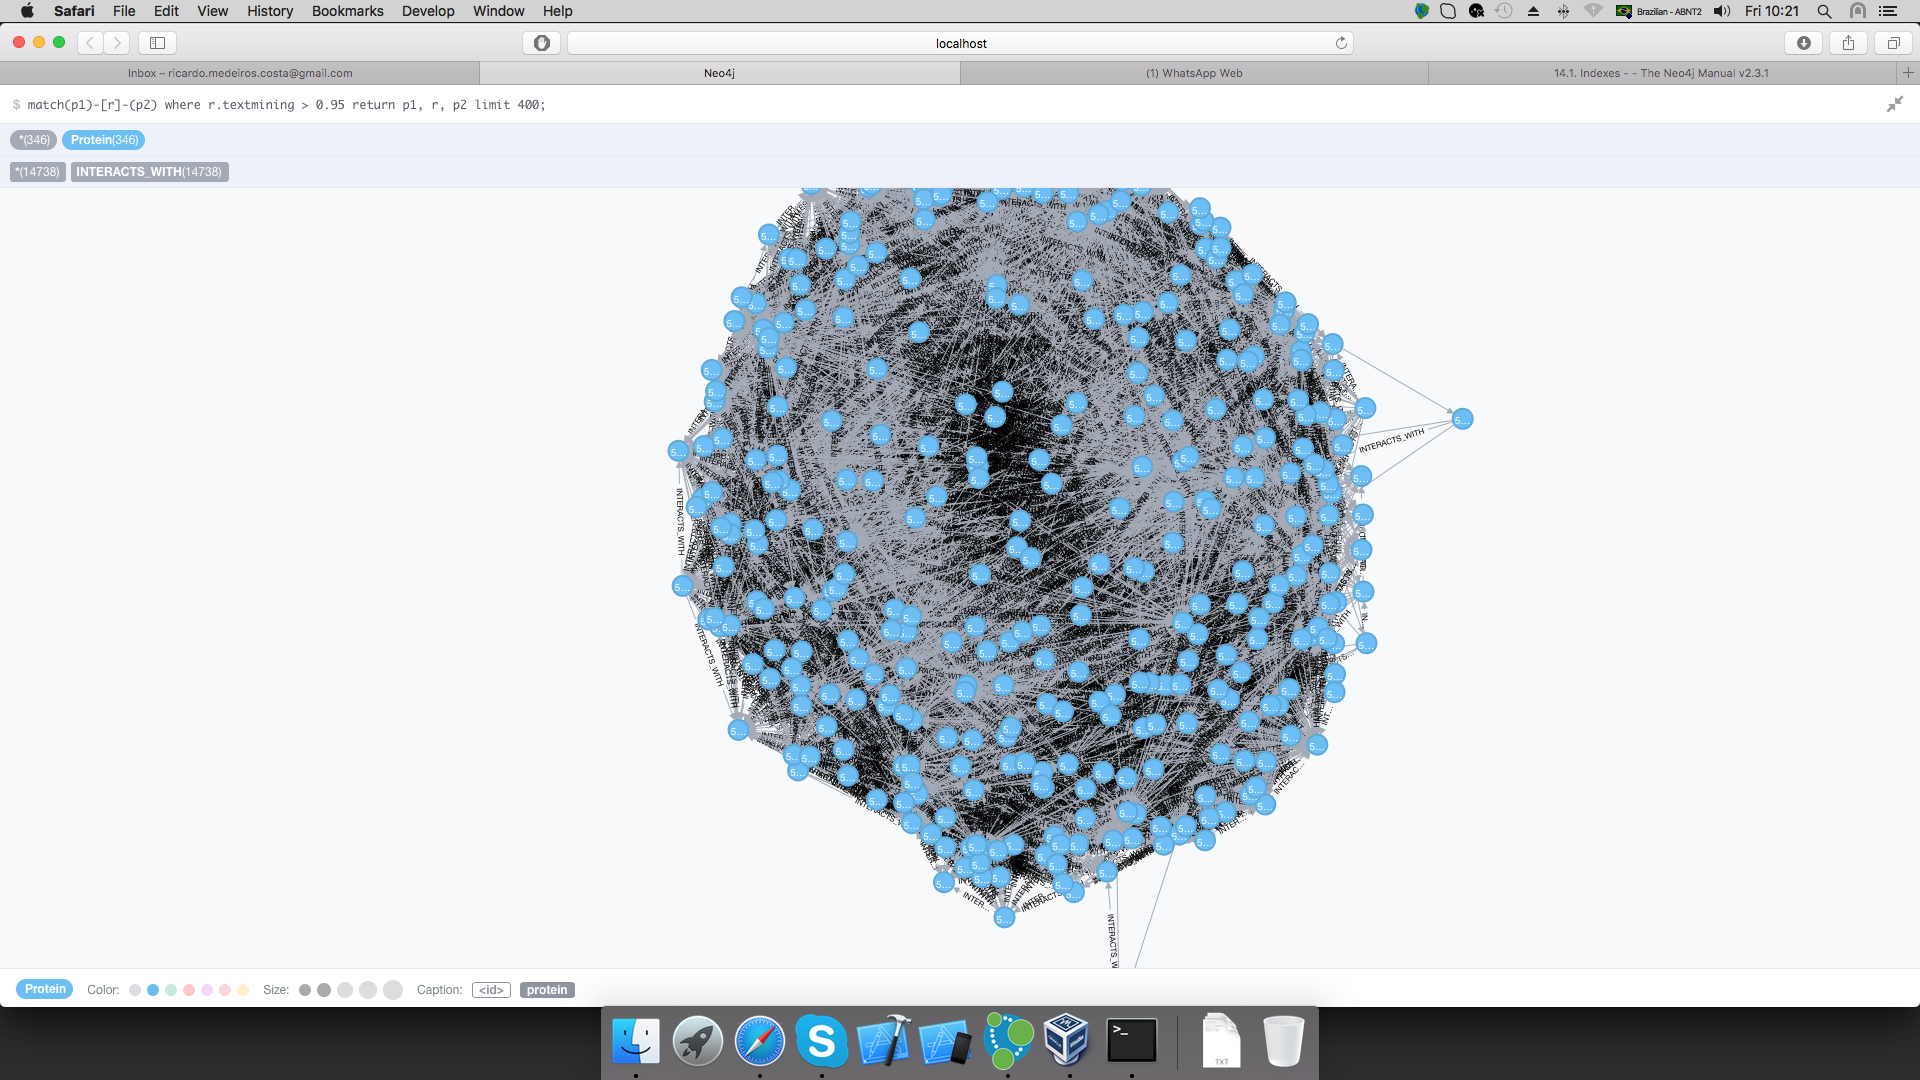
\includegraphics[width=1\textwidth]{4}
  \caption[4 - Filtrando Interações]{\textbf{Filtrando Interações}}
\end{figure}

\section{Contexto de uma Proteína}

\begin{lstlisting}[frame=single]
match(a {protein:'525254.HMPREF0072_2242'}
match(a)-[r]-(b)
return a, b
\end{lstlisting}

O resultado:
\begin{figure}[H]
  \centering
  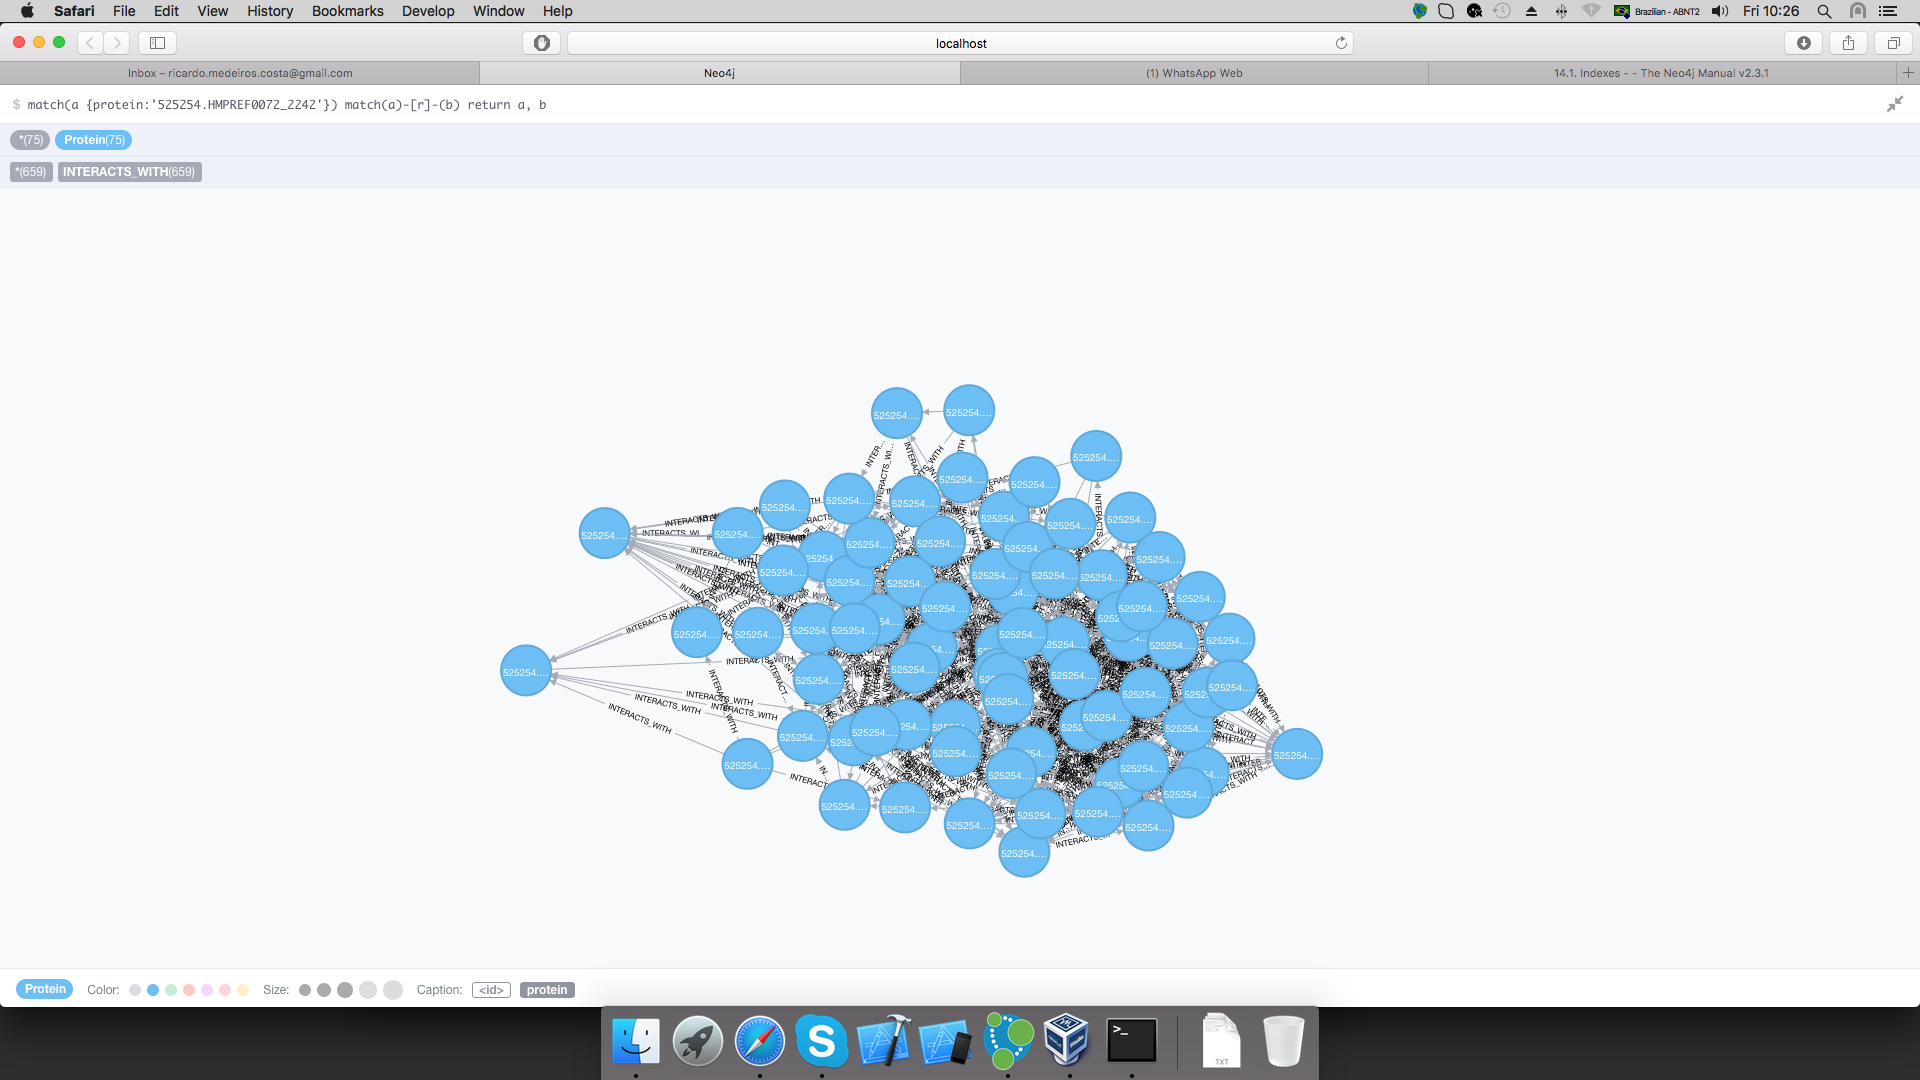
\includegraphics[width=1\textwidth]{5}
  \caption[5 - Context de uma Proteína]{\textbf{Contexto de uma Proteína}}
\end{figure} 

\section{Caminho Mais Curto}

\begin{lstlisting}[frame=single]
match (p1 {protein:''525254.HMPREF0072_2242''}), 
      (p2 {protein:''525254.HMPREF0072_0483''}),
sp = shortestPath((p1)-[r*]-(p2))
return sp;

\end{lstlisting}

O resultado:
\begin{figure}[H]
  \centering
  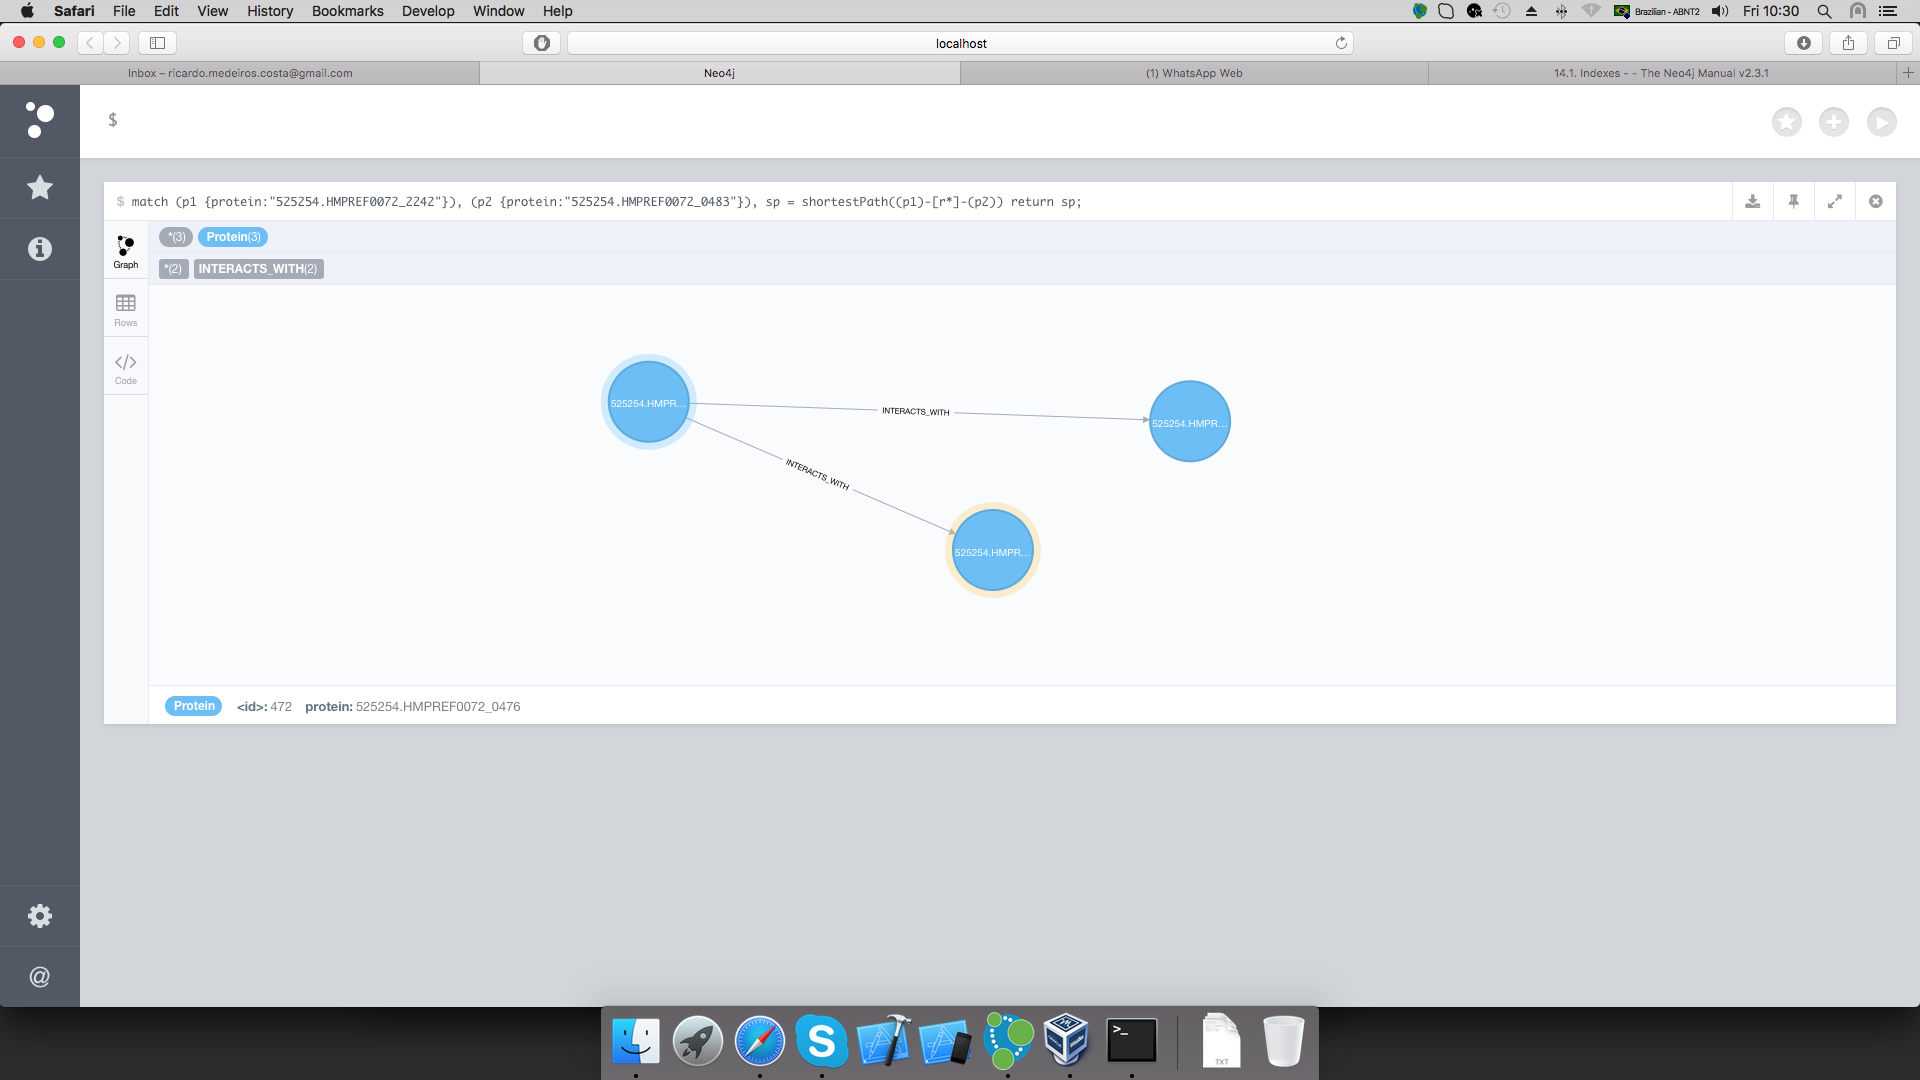
\includegraphics[width=1\textwidth]{6}
  \caption[6 - Caminho mais curto]{\textbf{Caminho mais curto}}
\end{figure}

\end{document}
